\subsection{Κατανόηση Αλγορίθμου}

Χωρίζουμε το αρχικό μας χωρίο σε τρία ανισομερή υπό-διαστήματα χρησιμοποιώντας τα σημεία $x_1$ και $x_2$.
Τα σημεία αυτά βρίσκονται πολύ κοντά το ένα με το άλλο, και χάρη στην υπόθεσή μας ότι η συνάρτηση που
εξετάζουμε είναι αυστηρά σχεδόν κυρτή, καταλαβαίνουμε ότι στην περίπτωση που τραβούσαμε μια εφαπτομένη 
στα δύο σημεία και στις δύο περιπτώσεις η συνάρτηση θα βρισκεται πάνω από την ευθεία αυτή. Έτσι 
συμπεραίνουμε ότι δεν μπορεί να υπάρξει ελάχιστο το οποίο να βρίσκεται πιο δεξιά από το $x_2$, στην 
περίπτωση που $f(x_1) < f(x_2)$, και αντίστοιχα δεν μπορεί να υπάρξει ελάχιστο το οποίο να βρίσκεται πιο
αριστερά από το $x_1$, στην περίπτωση που $f(x_1) >= f(x_2)$. Η μείωση του χωρίου αναζήτησης συνεχίζει
μέχρι να φτάσουμε σε χωρίο μικρότερο από μια σταθερά $l$. Σημαντικό να σημειωθεί ότι η ακρίβεια του 
αλγορίθμου μας δεν μπορεί να είναι μικρότερη από $2*\epsilon$. Αυτό συμβαίνει γιατί στο υποθετικό σενάριο
όπου παίρνουμε $l$ πολύ μικρό, γεγονός το οποίο αποτρέπει τον αλγόριθμο από το να σταματήσει, όταν το
χωρίο αναζήτησης γίνει ίσο του $2*\epsilon$ τότε δεν μπορούμε να κάνουμε καμία περαιτέρω ουσιώδη μείωση
του χωρίου αναζήτησης καθώς τα $x_1=\frac{a+b}{2}-\epsilon$ και $x_2=\frac{a+b}{2}+\epsilon$ θα συνεχίζουν 
να ορίζουν το ίδιο χωρίο αναζήτησης.

\subsection{Βήματα Αλγορίθμου}

\begin{enumerate}
    \item Ελέγχουμε αν $b - a < l$. Αν ισχύει, σταματάμε την αναζήτηση.
    \item Στην περίπτωση που δεν ισχύει, θέτουμε $x1=\frac{a+b}{2}-\epsilon$ και
    $x_2=\frac{a+b}{2}+\epsilon$.
    \item Αν $f(x_1) < f(x_2)$, θέτουμε $a_{k+1}=a_k$ και $b_{k+1}=x_{2k}$.
    \item Αλλιώς θέτουμε $a_(k+1)=x_(1k)$ και $b_(k+1)=b_k$.
    \item Μεταβαίνουμε στην επόμενη επανάληψη του αλγορίθμου $k=k+1$ και σταματάμε όταν
    $b_k - a_k < l$.
\end{enumerate}

\subsection{Υπολογισμοί αντικειμενικής συνάρτησης συναρτήσει του $\epsilon$}
Παρατηρούμε ότι για $\epsilon >= \frac{l}{2}$ ο αλγόριθμος αδυνατεί να τερματίσει. Αυτό συμβαίνει
επειδή στην οριακή περίπτωση όπου $\epsilon = \frac{l}{2}$ το καινούριο χωρίο αναζήτησης μπορεί να 
πάρει τιμή το πολύ $l$. Έτσι είναι αδύνατον για αυτή τη τιμή του χωρίου, και εννοείται για οποιαδήποτε 
μεγαλύτερή της, να πληρεί την προϋπόθεση λήξης του αλγορίθμου.

\begin{figure}[h] % h for 'here', you can also use t (top), b (bottom), or p (page)
    \centering
    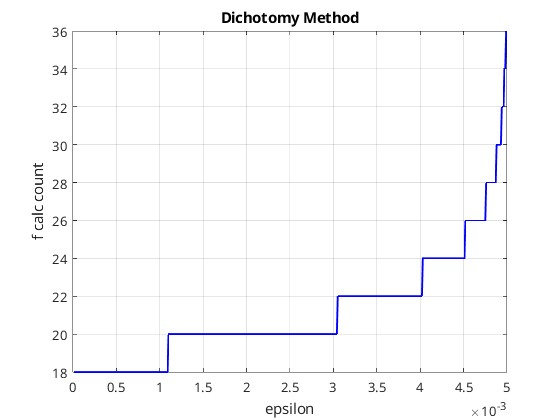
\includegraphics[width=0.5\textwidth]{media/dichotomyf1_1} % Image file without extension
\end{figure}

\subsection{Υπολογισμοί αντικειμενικής συνάρτησης συναρτήσει του $\lambda$}
Σε αυτή την περίπτωση μπορούμε να παρατηρήσουμε ότι οι υπολογισμοί της αντικειμενικής συνάρτησης
φθίνουν όσο μεγαλώνει το $\lambda$. Απαγορευτική τιμή εδώ αποτελεί η $\lambda <= 2*\epsilon$ καθώς
όπως και στην προηγούμενη περίπτωση δεν μπορούμε να μικρύνουμε το χωρίο αναζήτησης αρκετά έτσι ώστε να 
τερματίσει ο αλγόριθμος.

\begin{figure}[h] % h for 'here', you can also use t (top), b (bottom), or p (page)
    \centering
    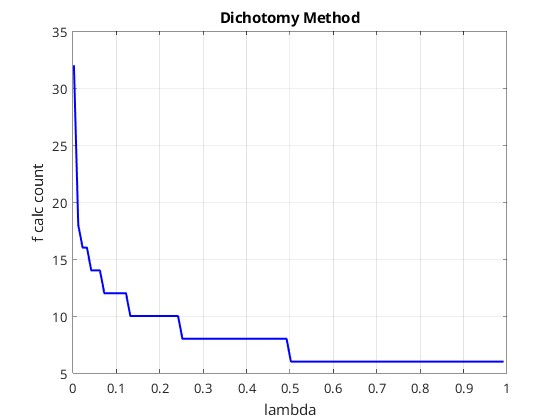
\includegraphics[width=0.5\textwidth]{media/dichotomyf1_2} % Image file without extension
\end{figure}

\subsection{Άκρα του διαστήματος αναζήτησης συναρτήσει του δείκτη επαναλήψεων}


\begin{figure}[h] % h for 'here', you can also use t (top), b (bottom), or p (page)
    \centering
    \includegraphics[width=0.5\textwidth]{media/dichotomyf1_3} % Image file without extension
\end{figure}